\documentclass[a4paper,8pt,twocolumn]{article}
\usepackage[UTF8]{ctex}
\usepackage{graphicx}
\usepackage{fancyhdr}
\usepackage{amsmath}
\usepackage{subcaption}
\usepackage{float}
\usepackage[
  left=2cm, 
  right=2cm,
  top=1.5cm,
  bottom=2.5cm
]{geometry}
\usepackage{pgfplots}
\usepackage{pgfplotstable}
\pgfplotsset{compat=1.18}
\usepackage{siunitx}
\usepackage{booktabs}
\usepackage{enumitem}
\usepackage{array}
\usepackage{tabularx}
% 定义可居中、可自动伸缩的 Y 列类型
\newcolumntype{Y}{>{\centering\arraybackslash}X}
\usepackage{amssymb} 

\sisetup{
  per-mode=symbol,
  separate-uncertainty = true
}

%================ 统一控制每个光谱图大小（大约一页可以排成 2×3） ================
\pgfplotsset{
  specplot/.style={
    width=0.9\columnwidth,     % 略窄少少，兩邊留白
    height=0.20\textheight,    % 高度大約 1/5 版心，高度明顯細好多
    scale only axis,
    grid=major,
    ymin=0,
    enlargelimits=false,
    xlabel={波长 / nm},
    ylabel={发光强度 / a.u.},
    title style={font=\small},
    label style={font=\small},
    ticklabel style={font=\scriptsize}
  }
}
%===============================================================================

\title{
  \textbf{\huge E4：基于光纤光谱仪的原子发射光谱实验}
}
\author{
  黄雨~24352027\\
\small 中山大学物理学院~广东~广州
}

\pagestyle{fancy}
\fancyhf{}
\fancyhead[C]{E4：基于光纤光谱仪的原子发射光谱实验}
\fancyfoot[C]{\thepage}

\begin{document}
\maketitle
\newpage

%%%%%%%%%%%%%%%%%%%%%%%%%%%%%%%%%%%%%%%%%%%%%%%%%%%%%%%%%%%%
\section{实验目的}

\begin{enumerate}
  \item 掌握光谱仪的基本结构与工作原理，了解单色仪、色散元件和探测器的作用。
  \item 观测钠原子发射光谱，理解碱金属原子光谱的一般规律与线系结构。
  \item 观测汞原子发射光谱，加深对外层电子与原子实相互作用以及自旋–轨道相互作用的认识。
  \item 利用光纤光谱仪测量多种实验室常用光源（汞灯、钠灯、氢氘灯、溴钨灯、LED 等）的发射光谱，并分析其光谱特征。
\end{enumerate}

%%%%%%%%%%%%%%%%%%%%%%%%%%%%%%%%%%%%%%%%%%%%%%%%%%%%%%%%%%%%
\section{实验仪器与装置}

\begin{itemize}
  \item 光纤光谱仪一台（光栅单色仪结构，内置一维 CCD 或 CMOS 线阵探测器，光谱响应范围约为 \SIrange{200}{850}{\nano\meter}，光谱分辨率约 \SI{2}{\nano\meter}）。
  \item 光纤探头及光纤接头组件，用于将待测光源光信号导入光谱仪。
  \item 多种气体放电光源：低压汞灯、低压钠灯、氢氘灯等。
  \item 连续光源：溴钨灯、白光 LED、红光 LED 等。
  \item LED 测量电路与采样电阻（阻值约 \SI{51}{\ohm}），通过测量采样电阻两端电压获得 LED 工作电流。
  \item 可调稳压电源、精密可调电阻、电流表或数字万用表。
  \item 计算机及配套光谱采集与分析软件（如 Ocean Optics 的 SpectraSuite 或杏林睿光 BSV 软件），用于光谱采集、时序测量与数据导出。
\end{itemize}

%%%%%%%%%%%%%%%%%%%%%%%%%%%%%%%%%%%%%%%%%%%%%%%%%%%%%%%%%%%%
\section{实验原理}

\subsection{碱金属原子光谱}

钠属于典型的碱金属原子，核外只有一个价电子，外层价电子在原子实（原子核与内层封闭壳层电子）形成的有效库仑势场中运动。与氢原子不同，原子实对价电子的作用场偏离点电荷库仑势，内层电子对核电荷产生屏蔽，使得能级结构不再完全氢样。

碱金属原子的光谱公式可写成
\begin{equation}
  \tilde{\nu}
  = R\!\left(
      \frac{1}{n_2^{*2}} - \frac{1}{n_1^{*2}}
    \right)
  = \frac{R}{(n'-\mu_{l'})^2}
    - \frac{R}{(n-\mu_l)^2},
  \tag{E4.1}
\end{equation}
其中，$\tilde{\nu}$ 为谱线波数，$R$ 为里德伯常数；$n',n$ 分别为始态和终态主量子数；$n^*_1,n^*_2$ 为有效主量子数；$l',l$ 为相应能级的轨道角动量量子数；$\mu_{l'},\mu_l$ 为量子缺（量子改正数或屏蔽常数），反映原子实对价电子库仑势的偏离程度。

根据玻尔理论，电子轨道越接近原子核，屏蔽越弱，所感受到的有效核电荷 $Z_{\mathrm{eff}}$ 越大，能级偏移越明显。对于贯穿轨道（电子轨道部分贯穿内层电子云），量子缺 $\mu$ 数值更大。一般而言，同一主量子数下，
\[
  \mu_s > \mu_p > \mu_d > \mu_f > \cdots,
\]
因此 $s$ 项能级偏离氢样能级最多，$p$ 项略小，$d$、$f$ 项更小。

钠原子光谱可分为四个线系：
\begin{itemize}
  \item 主线系：$\tilde{\nu} = np \rightarrow 3s \quad (n=3,4,5,\dots)$；
  \item 锐线系：$\tilde{\nu} = ns \rightarrow 3p \quad (n=4,5,6,\dots)$；
  \item 漫线系：$\tilde{\nu} = nd \rightarrow 3p \quad (n=3,4,5,\dots)$；
  \item 基线系：$\tilde{\nu} = nf \rightarrow 3d \quad (n=4,5,6,\dots)$。
\end{itemize}

对于任一线系，其谱线波数可写为
\begin{equation}
  \tilde{\nu}
  = A_{n'l'} - \frac{R}{(n-\mu_l)^2},
  \tag{E4.2}
\end{equation}
其中 $A_{n'l'}$ 为该线系的固定项（常数），由始态能级决定。

从钠原子光谱可归纳出碱金属原子光谱的一般特征：

\begin{enumerate}[label=(\arabic*)]
  \item \textbf{同一线系内谱线向短波端收敛。}\\
  随 $n$ 增大，能级间距减小，谱线在短波端逐渐逼近某一极限，最终趋于连续谱，这反映了高能级能级间距变密的趋势。

  \item \textbf{同一线系内高能级跃迁谱线的强度减弱。}\\
  由于激发原子到更高能级所需能量更大，粒子数目更少，因此线系中越靠近短波端的谱线强度越弱。

  \item \textbf{不同线系分布在不同光谱区域。}\\
  主线系中仅有 $3p \rightarrow 3s$ 的两条谱线（著名的钠双黄线）位于可见光区，其余谱线多在紫外区。由于主线系的下能级为基态（$3s_{1/2}$），当连续光谱通过钠蒸气时，会出现对应于主线系的吸收谱线——钠双黄线，波长分别约为 \SI{589.0}{\nano\meter} 和 \SI{589.6}{\nano\meter}，称为共振线。

  锐线系和漫线系的能级差较主线系小，其谱线除第一条（如 $4s\rightarrow 3p$ 和 $3d\rightarrow 3p$）位于红外区外，其余主要在可见区。基线系能级差更小，谱线集中在红外区。

  \item \textbf{自旋–轨道相互作用引起能级分裂和多重线结构。}\\
  $s$ 能级无简并，$p,d,f$ 等能级由于自旋–轨道耦合发生精细结构分裂，形成双重或复双重线。主线系与锐线系通常表现为双线结构，其中主线系双线的间隔由各 $p$ 能级的分裂决定，随 $n$ 增大，双线间波数差减小；锐线系则由 $3p$ 内层能级与各 $s$ 能级之间的跃迁产生，双线波数差近似相等。漫线系和基线系多为复双重线，谱线较为模糊。
\end{enumerate}

\subsection{单色仪及色散系统}

用于记录光谱的仪器统称为光谱仪，其核心部件是一台单色仪（monochromator）。单色仪的色散元件通常为棱镜或光栅，相应地称为棱镜单色仪与光栅单色仪。

光谱分辨能力常用分辨本领
\begin{equation}
  R = \frac{\lambda}{\Delta\lambda}
  \tag{E4.3}
\end{equation}
来描述，其中 $\lambda$ 为两条谱线的平均波长，$\Delta\lambda$ 为它们的波长差。当一条谱线的中心极大与另一条谱线的第一极小恰好重合时，两条谱线刚好能被分辨开。

\subsubsection{棱镜单色仪}

棱镜单色仪的色散元件为棱镜，其色散能力可用角色散 $d\theta/d\lambda$ 描述。对于足够接近的两条谱线，有
\begin{equation}
  \frac{d\theta}{d\lambda}
  \approx \frac{\Delta\theta}{\Delta\lambda}
  = \frac{\theta_2-\theta_1}{\lambda_2-\lambda_1} ,
  \tag{E4.4}
\end{equation}
又有
\begin{equation}
  \frac{d\theta}{d\lambda}
  = \frac{d\theta}{dn} \cdot \frac{dn}{d\lambda},
  \tag{E4.5}
\end{equation}
其中 $d\theta/dn$ 只与棱镜几何形状有关，$dn/d\lambda$ 为色散率，其值随波长减小而增大。紫外区常用石英棱镜，可见区常用玻璃棱镜，不同波段往往需要更换棱镜，使用上不够方便。

\subsubsection{光栅单色仪}

光栅单色仪以平面透射或反射光栅为色散元件。平面透射光栅的衍射条件为
\begin{equation}
  k\lambda = d\sin\theta,
  \quad k=0,1,2,\dots,
  \tag{E4.6}
\end{equation}
其中 $d$ 为光栅常数，$\theta$ 为衍射角。当入射光不垂直光栅平面而与法线成 $i$ 角时，光栅方程写为
\begin{equation}
  k\lambda = d(\sin\theta + \sin i).
  \tag{E4.7}
\end{equation}

对式 \eqref{E4.7} 对 $\lambda$ 求微分，可得角色散
\begin{equation}
  \frac{d\theta}{d\lambda}
  = \frac{k}{d\cos\theta}.
  \tag{E4.8}
\end{equation}
由此可见：
\begin{itemize}
  \item 在 $\Delta\lambda$ 很小的条件下，$\Delta\theta \propto k$，即衍射级次越高，色散越大；
  \item $\Delta\theta \propto 1/d$，光栅刻线密度越高（$d$ 越小），色散越大；
  \item 在 $\cos\theta$ 变化不大的范围内，$d\theta/d\lambda$ 近似为常数，即光栅的色散近似线性。
\end{itemize}

现代光谱仪中广泛使用反射式全息光栅，具有刻线密度高、杂散光低、重复性好的优点。光栅单色仪一级谱的分辨率可达 \SI{0.02}{\nano\meter}，能分辨如钠双黄线这样的细小波长差。

\subsection{光栅光谱仪与光学多道分析仪}

将单色仪输出的谱线用探测器记录即可形成光栅光谱仪。按照探测方式不同，可分为：
\begin{itemize}
  \item 采用光电倍增管或光电二极管的扫描式光谱仪：每次只能记录一条谱线，灵敏度极高，适合微弱光信号测量；
  \item 采用线阵 CCD 或 CMOS 的光学多道分析仪（Optical Multichannel Analyzer，OMA）：可同时记录一个波长段内的全部谱线，测量速度快，适合常规发射光谱测量。
\end{itemize}

典型反射光栅光谱仪的光路包括：入射狭缝（位于准直镜焦平面）、准直镜、反射光栅、成像物镜、出射狭缝和光电探测器等。通过转动光栅或反射镜扫描不同衍射角即可实现波长扫描。

\subsection{光纤光谱仪}

光纤光谱仪内部结构与传统光栅光谱仪类似，但所有光学元件与光栅位置均为固定，狭缝宽度与光谱范围在出厂时已经标定，用户无法调整。典型结构包括：
\begin{enumerate}
  \item 光纤连接器与入射狭缝；
  \item 准直镜与反射光栅；
  \item 聚焦镜与探测器前透镜；
  \item 一维 CCD（或 CMOS）线阵探测器；
  \item USB 数据接口和控制电子学。
\end{enumerate}

光纤光谱仪输出的是 CCD 计数值 $S(\lambda)$ 随波长的变化曲线。根据需要可进一步计算透射谱 $T(\lambda)$、反射谱 $R(\lambda)$、吸收谱 $A(\lambda)$ 或经标定后的光强谱 $I(\lambda)$ 等。积分时间（曝光时间）决定单次采集的信号强度，需在避免饱和的前提下尽量增大；多次平均可减小随机噪声，使光谱曲线更平滑。

%%%%%%%%%%%%%%%%%%%%%%%%%%%%%%%%%%%%%%%%%%%%%%%%%%%%%%%%%%%%
\section{实验内容与步骤}

\subsection{总体任务}

本实验利用光纤光谱仪完成以下几项测量与分析任务：
\begin{enumerate}[label=\arabic*)]
  \item 测量多种光源（低压汞灯、低压钠灯、氢氘灯、溴钨灯、各色 LED 灯）的发射光谱，比较线谱与连续谱以及不同光源间光谱结构的差异。
  \item 测量汞灯 \SI{546}{\nano\meter} 谱线和钠灯 \SI{589}{\nano\meter} 谱线在点亮后的强度随时间变化曲线，研究放电灯的预热与稳定过程。
  \item 测量白光 LED（峰值约 \SI{545}{\nano\meter}）和红光 LED（峰值约 \SI{627}{\nano\meter}）的峰值发光强度随工作电流的变化关系，得到其电致发光特性曲线，并分析发光效率与线性范围。
\end{enumerate}

\subsection{光谱测量步骤（发射光谱）}

以下以海洋光学光纤光谱仪及 SpectraSuite 软件为例说明具体操作方法：

\begin{enumerate}[label=\arabic*)]
  \item 打开计算机，启动光谱仪控制软件（如 SpectraSuite），确认光谱仪已通过 USB 接口正确连接。
  \item 点亮待测光源，将光纤探头固定于支架上，对准光源发光区域，适当调整距离与角度，使入射光强适中。
  \item 在软件中选择实时采集模式，设置积分时间（如 \SI{1}{\milli\second} 起步），调整平均次数（如 3 次）和其他采集参数，使光谱峰值计数在探测器动态范围之内而不过饱和。
  \item 记录背景光谱（关光源或遮挡光路），用于后续背景扣除。
  \item 对低压汞灯、低压钠灯、氢氘灯、溴钨灯、各色 LED 等光源逐一重复上述步骤，采集并保存各自的发射光谱数据和光谱曲线截图。
  \item 在数据分析中识别各个显著谱线的波长位置与相对强度，比较不同光源的线谱结构和连续背景。
\end{enumerate}

若使用杏林睿光光谱仪，则在 BSV 软件中完成类似的采集操作，并通过“文件 $\to$ 导出数据”功能将光谱保存为文本文件，后续用 Origin、Matlab 或 Python 等工具进行处理。

\subsection{时序测量步骤（谱线强度随时间变化）}

本部分测量汞灯 \SI{546}{\nano\meter} 谱线和钠灯 \SI{589}{\nano\meter} 谱线在点亮后的强度随时间变化。

\begin{enumerate}[label=\arabic*)]
  \item 将光纤探头固定在合适位置，对准待测光源，使光谱仪在对应谱线波长附近能够获得较高信噪比。
  \item 在软件中进入时序测量模式（“Scope Time”或“时序图”界面），指定单波长监测模式，如选择波长 $\lambda=\SI{546.18}{\nano\meter}$ 或 $\lambda=\SI{589}{\nano\meter}$。
  \item 设定时间采样间隔和总测量时间（如每隔数百毫秒采样一次，总时间约 3--5 分钟），同时设置合理的积分时间与平均次数。
  \item 开始时序采集的同时点亮放电灯，记录谱线强度 $S(t)$ 随时间的变化，直至光源输出基本稳定。
  \item 停止采集，保存时序数据与强度–时间曲线图，用于分析灯的预热时间、稳定输出阶段和可能的漂移。
\end{enumerate}

\subsection{LED 发光强度–电流特性测量}

以白光 LED 和红光 LED 为测量对象，通过采样电阻测定工作电流，并利用光纤光谱仪记录对应波段峰值强度：

\begin{enumerate}[label=\arabic*)]
  \item 按照电路图将 LED 与采样电阻（\SI{51}{\ohm}）串联接入可调电源，加入限流保护，确保最大电流 $I_{\max}<\SI{40}{\milli\ampere}$。
  \item 将光纤探头固定在支架上，对准被测 LED，保持几何位置固定不变，避免测量过程中移动导致耦合光强变化。
  \item 在光谱仪软件中选择连续采集模式，调节积分时间和平均次数，使 LED 光谱峰值不饱和。
  \item 由 $I=U_R/R$ 计算 LED 工作电流，其中 $U_R$ 为采样电阻两端电压，$R$ 为采样电阻阻值（\SI{51}{\ohm}）。
  \item 以约 \SI{2}{\milli\ampere} 为步长，从 $I\approx 0$ 开始逐步增大至约 \SI{40}{\milli\ampere}，在每一个电流点上记录对应的光谱，并读取 LED 峰值波长附近的光强（如白光 LED 的 \SI{545}{\nano\meter} 附近，红光 LED 的 \SI{627}{\nano\meter} 附近）。
  \item 绘制白光 LED 和红光 LED 的峰值光强 $I_{\lambda}$ 随驱动电流 $I$ 的变化曲线，分析在小电流区域的近线性关系及大电流区域可能出现的饱和与热效应。
\end{enumerate}

%%%%%%%%%%%%%%%%%%%%%%%%%%%%%%%%%%%%%%%%%%%%%%%%%%%%%%%%%%%%
\section{实验记录与分析}

\subsection{常见光源发射光谱特征}

实验中测得的几种典型光源的发射光谱具有以下特征：

\begin{itemize}
  \item \textbf{低压汞灯：} 光谱以数条强线谱为主，典型的绿线位于 \SI{546}{\nano\meter} 附近，此外在蓝紫、黄等波段也有若干明显谱线，是标准的线状发射光谱。
  \item \textbf{低压钠灯：} 以钠双黄线为最显著特征，位于约 \SI{589.0}{\nano\meter} 和 \SI{589.6}{\nano\meter}，其余谱线相对较弱。由于本实验光谱分辨率约为 \SI{2}{\nano\meter}，在测得光谱中钠双黄线可能难以完全分开。
  \item \textbf{氢氘灯：} 在紫外至可见区域可观察到若干氢原子 Balmer 系谱线，如 H$\alpha$、H$\beta$ 等；光谱中还叠加有连续背景，是常用的紫外–可见标准光源。
  \item \textbf{溴钨灯：} 近似黑体辐射连续光谱，在可见和近红外区光强随波长逐渐增加，整体光谱较为平滑，无孤立尖锐谱线。
  \item \textbf{各色 LED：} 白光 LED 的光谱通常由蓝光芯片发射峰与荧光粉转换后的宽带黄–红光叠加构成，呈宽带连续分布；红光、绿光等单色 LED 多呈单峰或少数窄峰结构，其峰值位置对应半导体材料带隙。
\end{itemize}

%======================= 单独绘制 6 个光谱图，大小统一 =======================

\begin{figure}[htbp]
  \centering
  \begin{tikzpicture}
  \begin{axis}[
      specplot,
      title={低压汞灯发射光谱}
  ]
    \addplot[mark=none,green!60!black,thick,smooth]
      table[x index=0,y index=1]{低压汞灯.txt};
  \end{axis}
  \end{tikzpicture}
  \caption{低压汞灯发射光谱}
\end{figure}

\begin{figure}[htbp]
  \centering
  \begin{tikzpicture}
  \begin{axis}[
      specplot,
      title={低压钠灯发射光谱}
  ]
    \addplot[mark=none,red,thick,smooth]
      table[x index=0,y index=1]{低压钠灯.txt};
  \end{axis}
  \end{tikzpicture}
  \caption{低压钠灯发射光谱}
\end{figure}

\begin{figure}[htbp]
  \centering
  \begin{tikzpicture}
  \begin{axis}[
      specplot,
      title={氢氘灯发射光谱}
  ]
    \addplot[mark=none,blue,thick,smooth]
      table[x index=0,y index=1]{氢氘灯.txt};
  \end{axis}
  \end{tikzpicture}
  \caption{氢氘灯发射光谱}
\end{figure}

\begin{figure}[htbp]
  \centering
  \begin{tikzpicture}
  \begin{axis}[
      specplot,
      title={溴钨灯发射光谱}
  ]
    \addplot[mark=none,black,thick,smooth]
      table[x index=0,y index=1]{溴钨灯.txt};
  \end{axis}
  \end{tikzpicture}
  \caption{溴钨灯发射光谱}
\end{figure}

\begin{figure}[htbp]
  \centering
  \begin{tikzpicture}
  \begin{axis}[
      specplot,
      title={红光 LED 发射光谱}
  ]
    \addplot[mark=none,red,thick,smooth]
      table[x index=0,y index=1]{红.txt};
  \end{axis}
  \end{tikzpicture}
  \caption{红光 LED 发射光谱}
\end{figure}

\begin{figure}[htbp]
  \centering
  \begin{tikzpicture}
  \begin{axis}[
      specplot,
      title={绿光 LED 发射光谱}
  ]
    \addplot[mark=none,green!70!black,thick,smooth]
      table[x index=0,y index=1]{绿.txt};
  \end{axis}
  \end{tikzpicture}
  \caption{绿光 LED 发射光谱}
\end{figure}

%====================================================================

\subsection{钠原子光谱与线系判别}

根据前述线系定义，可利用实验测得的钠灯谱线对照理论分析：

\begin{itemize}
  \item 置于可见光区、强度最大的 \SI{589}{\nano\meter} 附近双线属于主线系 $np\rightarrow 3s$ 中的 $3p\rightarrow 3s$ 跃迁，是主线系的第一组线（共振线）。
  \item 若在实验中（或更高分辨率仪器下）观察到位于红外方向、波长较长且强度较弱的谱线，可将其归为锐线系 $ns\rightarrow 3p$ 的第一条线（如 $4s\rightarrow 3p$）。
  \item 漫线系与基线系的谱线多分布在红外区，在本实验光谱响应范围边缘附近可能仅能观察到部分谱线，且由于精细结构和复双重线的叠加，谱线轮廓较为模糊。
\end{itemize}

综合分析可验证钠原子发射光谱中不同线系的分布规律及其强度变化特征。

\subsection{汞绿线与钠双黄线强度随时间的演化}

放电灯在点亮瞬间电极和气体尚未达到热平衡，气体压强、电离度和放电状态随时间变化，导致特定谱线强度随时间逐渐变化直至稳定。

实验的结果为：

\begin{itemize}
  \item \textbf{汞灯 \SI{546}{\nano\meter} 绿线：} 在刚点亮时有尖峰，随继光强较弱，随后随时间迅速上升，经过数十秒到数分钟后逐渐趋于稳定。曲线呈现上升后平台的特征，反映了灯内气压与汞蒸气浓度逐渐稳定的过程。
  \begin{figure}[htbp]
  \centering
  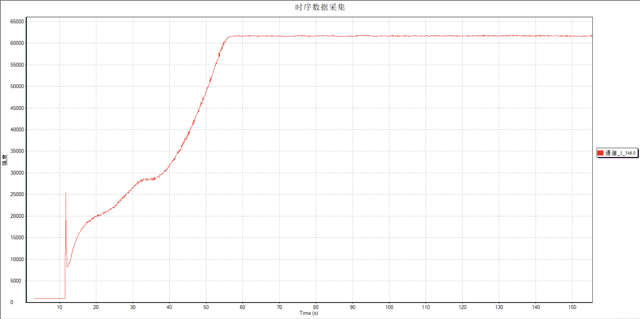
\includegraphics[width=0.95\columnwidth]{汞灯时序.png}
  \caption{汞灯 \SI{546}{\nano\meter} 谱线强度随时间变化}
  \end{figure}
  \item \textbf{钠灯 \SI{589}{\nano\meter} 谱线：} 同样表现出从弱到强的变化过程，预热时间可能比汞灯更长。部分钠灯在预热阶段光色与稳定阶段不同，光谱也随之演化，最终以钠双黄线为主。
  \begin{figure}[htbp]
  \centering
  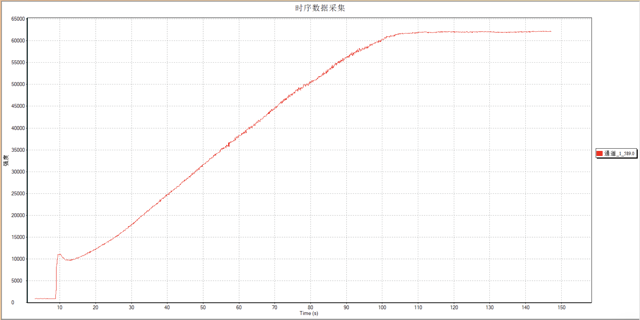
\includegraphics[width=0.95\columnwidth]{钠灯时序.png}
  \caption{钠灯 \SI{589}{\nano\meter} 谱线强度随时间变化}
  \end{figure}
\end{itemize}

通过时序测量曲线可以估计放电灯的预热时间和达到稳定输出所需的时间，对实际光学实验中光源的使用具有重要参考意义。

\subsection{LED 峰值光强–电流特性}

对白光 LED 和红光 LED 测得的峰值光强随电流变化曲线一般具有以下定性特点：

\begin{itemize}
  \item 在较小电流区域，LED 峰值光强 $I_{\lambda}$ 近似与驱动电流 $I$ 成正比，即
  \[
    I_{\lambda} \propto I,
  \]
  发光效率基本恒定，器件工作在线性区。
  \item 随电流进一步增大，结温升高，量子效率和出光效率下降，光强–电流曲线会逐渐偏离严格线性关系，可能出现趋于饱和甚至略有下降的趋势。
  \item 白光 LED 的光谱各组成峰（蓝光和宽带黄光）随电流变化的比例可能略有不同，导致整体色坐标略有漂移；红光 LED 谱线较窄，但峰位随结温升高可能向长波方向发生微小红移。
\end{itemize}
% 白光 LED 峰值光强-电流特性
\begin{figure}[htbp]
  \centering
  \begin{tikzpicture}
  \begin{axis}[
      specplot,
      title={白光 LED 峰值光强-电流特性},
      xlabel={电流 $I$ / mA},
      ylabel={峰值光强 / a.u.}
  ]
    \addplot[
      mark=*,
      red,
      thick,
      smooth
    ] coordinates {
      (0.00,  946)
      (2.06, 1639)
      (4.00, 3937)
      (5.78, 4696)
      (7.76, 5461)
      (9.71, 6519)
      (11.82, 7504)
      (13.71, 8295)
      (15.98, 8967)
      (17.69, 9261)
      (19.59, 9537)
      (21.75,10041)
      (23.71,10285)
    };
  \end{axis}
  \end{tikzpicture}
  \caption{白光 LED 峰值光强随电流变化曲线}
\end{figure}
\begin{table}[H]
\centering
\caption{白光 LED（$\lambda \approx 545\,\mathrm{nm}$）峰值光强与电流}
\begin{tabular}{ccc}
\toprule
$U/\mathrm{mV}$ & $I/\mathrm{mA}$ & 强度 / a.u. \\
\midrule
0    & 0.00 & 946   \\
105  & 2.06 & 1639  \\
204  & 4.00 & 3937  \\
295  & 5.78 & 4696  \\
396  & 7.76 & 5461  \\
495  & 9.71 & 6519  \\
603  & 11.82 & 7504  \\
699  & 13.71 & 8295  \\
815  & 15.98 & 8967  \\
902  & 17.69 & 9261  \\
999  & 19.59 & 9537  \\
1109 & 21.75 & 10041 \\
1209 & 23.71 & 10285 \\
\bottomrule
\end{tabular}
\end{table}

% 红光 LED 峰值光强-电流特性
\begin{figure}[htbp]
  \centering
  \begin{tikzpicture}
  \begin{axis}[
      specplot,
      title={红光 LED 峰值光强-电流特性},
      xlabel={电流 $I$ / mA},
      ylabel={峰值光强 / a.u.}
  ]
    \addplot[
      mark=*,
      blue,
      thick,
      smooth
    ] coordinates {
      (0.00,  967)
      (2.08, 1059)
      (3.92, 1147)
      (5.75, 1212)
      (7.84, 1310)
      (10.00,1344)
      (11.94,1405)
      (13.75,1521)
      (15.59,1576)
      (17.57,1691)
      (19.49,1733)
      (21.57,1519)
      (23.86,1326)
      (25.41,1403)
      (27.39,1621)
      (29.63,2070)
    };
  \end{axis}
  \end{tikzpicture}
  \caption{红光 LED 峰值光强随电流变化曲线}
\end{figure}
\begin{table}[H]
\centering
\caption{红光 LED（$\lambda \approx 627\,\mathrm{nm}$）峰值光强与电流}
\begin{tabular}{ccc}
\toprule
$U/\mathrm{mV}$ & $I/\mathrm{mA}$ & 强度 / a.u. \\
\midrule
0    & 0.00 & 967  \\
106  & 2.08 & 1059 \\
200  & 3.92 & 1147 \\
293  & 5.75 & 1212 \\
400  & 7.84 & 1310 \\
510  & 10.00 & 1344 \\
609  & 11.94 & 1405 \\
701  & 13.75 & 1521 \\
795  & 15.59 & 1576 \\
896  & 17.57 & 1691 \\
994  & 19.49 & 1733 \\
1100 & 21.57 & 1519 \\
1217 & 23.86 & 1326 \\
1296 & 25.41 & 1403 \\
1397 & 27.39 & 1621 \\
1511 & 29.63 & 2070 \\
\bottomrule
\end{tabular}
\end{table}


%%%%%%%%%%%%%%%%%%%%%%%%%%%%%%%%%%%%%%%%%%%%%%%%%%%%%%%%%%%%
\section{思考题}

\begin{enumerate}
  \item \textbf{钠原子光谱有哪些特征？从光谱图上如何判断各谱线所属线系？}\\[0.3em]
  钠原子光谱具有典型的线系结构，包括主线系、锐线系、漫线系和基线系。主线系中最显著的是位于可见光区的钠双黄线（约 \SI{589.0}{\nano\meter} 和 \SI{589.6}{\nano\meter}），其余主线系谱线多在紫外区；锐线系、漫线系分布在可见与近红外区；基线系主要位于红外区。根据谱线所在波段、相对强度以及能级差大小，可以结合理论跃迁式 $\tilde{\nu}=np\rightarrow 3s$、$ns\rightarrow 3p$、$nd\rightarrow 3p$ 等，将实测谱线归属到相应线系中。主线系谱线较强且短波端收敛明显，锐线系谱线轮廓清晰，漫线系与基线系谱线较为模糊。

  \item \textbf{什么是标准谱线？}\\[0.3em]
  标准谱线是指波长已被精确测定且在空间和时间上具有良好稳定性、重复性，常被用作光谱仪标定和波长基准的谱线。例如汞灯的 \SI{546.07}{\nano\meter} 绿线、\SI{435.83}{\nano\meter} 蓝线以及钠原子的双黄线等，都是常用的标准谱线。利用标准谱线可以建立光谱仪像素位置与波长之间的定量对应关系，提高波长测量的准确度。

  \item \textbf{光谱仪使用前为什么要进行标定？}\\[0.3em]
  光谱仪的光学系统和探测器在制造和安装过程中不可避免存在误差，环境温度、机械振动和长期使用也会引入波长漂移和响应变化。若不进行标定，软件给出的波长轴与真实波长之间可能存在系统偏差，导致谱线识别和定量分析出现误差。因此，在正式测量前需要利用标准光源（如汞灯、氢灯、钠灯等）发出的标准谱线对光谱仪进行波长标定和强度响应校正，以保证测量结果的准确性和可重复性。
\end{enumerate}

%%%%%%%%%%%%%%%%%%%%%%%%%%%%%%%%%%%%%%%%%%%%%%%%%%%%%%%%%%%%

\clearpage
\onecolumn
\section*{教师签名页}
\begin{figure}[htbp]
  \centering
  
\includegraphics[width=0.95\columnwidth]{签名页.png}
  \caption{教师签名页}
\end{figure}

\end{document}